% !TEX root = ../main.tex

\chapter{Influence Among Artists}

Some artists can list a dozen or more other artists who they say influenced their own musical work. It has also been suggested that influence can be measured by the degree of similarity between song characteristics, such as structure, rhythm, or lyrics. In this chapter, a directed network of influencers and followers is established according to ``influence\_data'' reported by the artists themselves, as well as the opinions of industry experts. In addition, the similarity of song characteristics among different artists is analysed to reflect the influence in another way. After a brief comparison between two influence networks, it may lead to some interesting results.

\section{A directed network of influencers and followers}

According to ``influence\_data'' and preceding entropy weight analysis, a directed network of influencers and followers can be established with each artist having a weight coefficient. For convenience of analysis and visualization, a sub-network including top 100 influential artists is built and plotted in Figure \ref{fig:influence}.\par

\begin{figure}
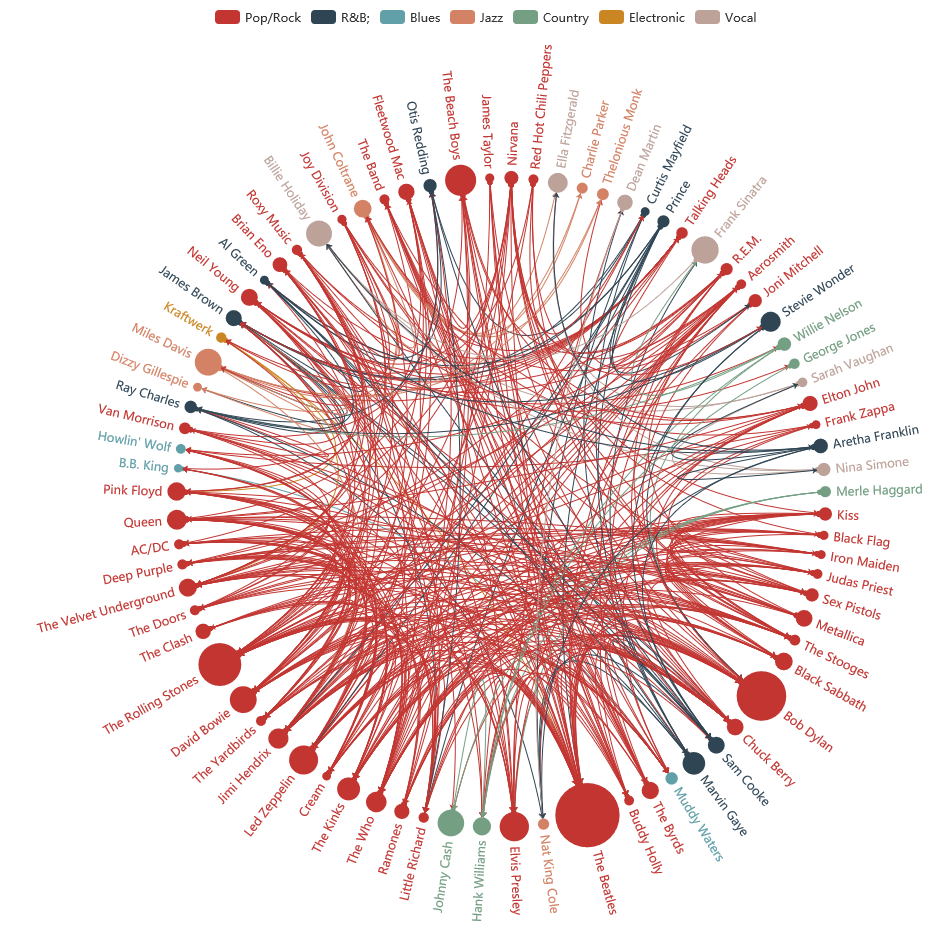
\includegraphics[width=1.25\textwidth]{figures/xdq/influence.png}
\setlength{\leftskip}{0pt plus 1fil minus \marginparwidth}
\setlength{\rightskip}{\leftskip}
\caption{A directed network of influencers and followers}
\label{fig:influence}
\end{figure}

In Figure \ref{fig:influence}, the size of a node represents the influence score of an artist and the direction of an arrow is from a follower to an influencer. It is clear that most of the top 100 artists are from genre Pop/Rock (in red colour). The Beatles, Bob Dylan, and The Rolling Stones come top 3 influential artists, which consists well with the previous analysis and the reality. The Beatles is regarded as the most influential band of all time; Bob Dylan is one of the greatest songwriters, and The Rolling Stone is one of the most famous rock bands. It is noticeable that in this network, the link between two artists has a specific direction, that is to say, one is the influencer while the other is influenced, which is different from similarity analysis. Moreover, an influencer can also be a follower, giving the fact that the most influential artist The Beatles is also influenced by ``The Band'' and Bob Dylan. This reveals the mutual influence of artists on each other.

\section{Similarity of music features among artists}

Similarity between song characteristics can also reflect musical influence among artists. To be clear, two artists sharing the similar music style would have a greater chance to be influenced by each other. This section is aimed to build another influence network based on similarity analysis.

\subsection{Euclidean similarity}

In $\mathbb{R}^n$, the Euclidean distance $||x-y||_2$ between two vectors $x = (x_1, x_2, ..., x_n)$ and $y = (y_1, y_2, ... , y_n)$ is always defined. It corresponds to the $L_2$-norm $||.||_2$ of the difference $x$--$y$ between the two vectors. It can be computed as:
\begin{equation}
\|x-y\|_{2}=\sqrt{\sum_{i=1}^{n}\left(x_{i}-y_{i}\right)^{2}}=\sqrt{\left(x_{1}-y_{1}\right)^{2}+\left(x_{2}-y_{2}\right)^{2}+\ldots+\left(x_{n}-y_{n}\right)^{2}}
\end{equation}
Here, PC1--PC7 are 7 major components reflecting the music style, so the Euclidean distance between two artists' music characteristics is:
\begin{equation}
dist_{i,j}=\sqrt{\sum_{k=1}^{7}\left(P C_{k}^{i}-P C_{k}^{j}\right)^{2}}
\end{equation}
In order to get a similarity coefficient ranging from 0 to 1, we define Euclidean similarity as:
\begin{equation}
Sim_{L2}^{i,j}=\frac{1}{dist_{i, j}+1}
\end{equation}

\subsection{Cosine similarity}

In data analysis, cosine similarity is a measure of similarity between two sequences of numbers. For defining it, the sequences are viewed as vectors in an inner product space, and the cosine similarity is defined as the cosine of the angle between them, that is, the dot product of the vectors divided by the product of their lengths, as shown in Equation \eqref{cosine}. It follows that the cosine similarity does not depend on the magnitudes of the vectors, but only on their angle. The cosine similarity always belongs to the interval [-1,1]. 

\begin{equation}
Sim_{cos}^{i, j}=\frac{\sum_{k=1}^{7} P C_{k}^{i} P C_{k}^{j}}{\sqrt{\sum_{k=1}^{7}\left(P C_{k}^{i}\right)^{7}} \sqrt{\sum_{k=1}^{7}\left(P C_{k}^{j}\right)^{2}}}
\label{cosine}
\end{equation}

\subsection{Similarity of music characteristics among artists}

The data set ``data\_by\_artis'' provides us with more than 10 musical features of each artist, such as danceability, tempo, loudness and etc. After PCA and entropy weight analysis, we select 100 most influential artists to measure their similarities among each other. Euclidean similarity could reflect the distance between 2 vectors in the space, while some problems may occur when two vectors are close to the original point but in totally different directions. Cosine similarity is useful to reveal the similarity in directions, neglecting the information of length. It would be more reasonable to consider both Euclidean similarity and cosine similarity in this case. We define that two artists share the similar music style (have a potential to influence each other), when:
\begin {equation}
Sim_{cos}^{i, j}>0.7 \qquad \text{and} \qquad Sim_{L2}^{i,j}>0.7
\end{equation}

Under such criterion, a new influence network is established based on similarity analysis, as shown in Figure \ref{fig:similarity}.

\begin{figure}
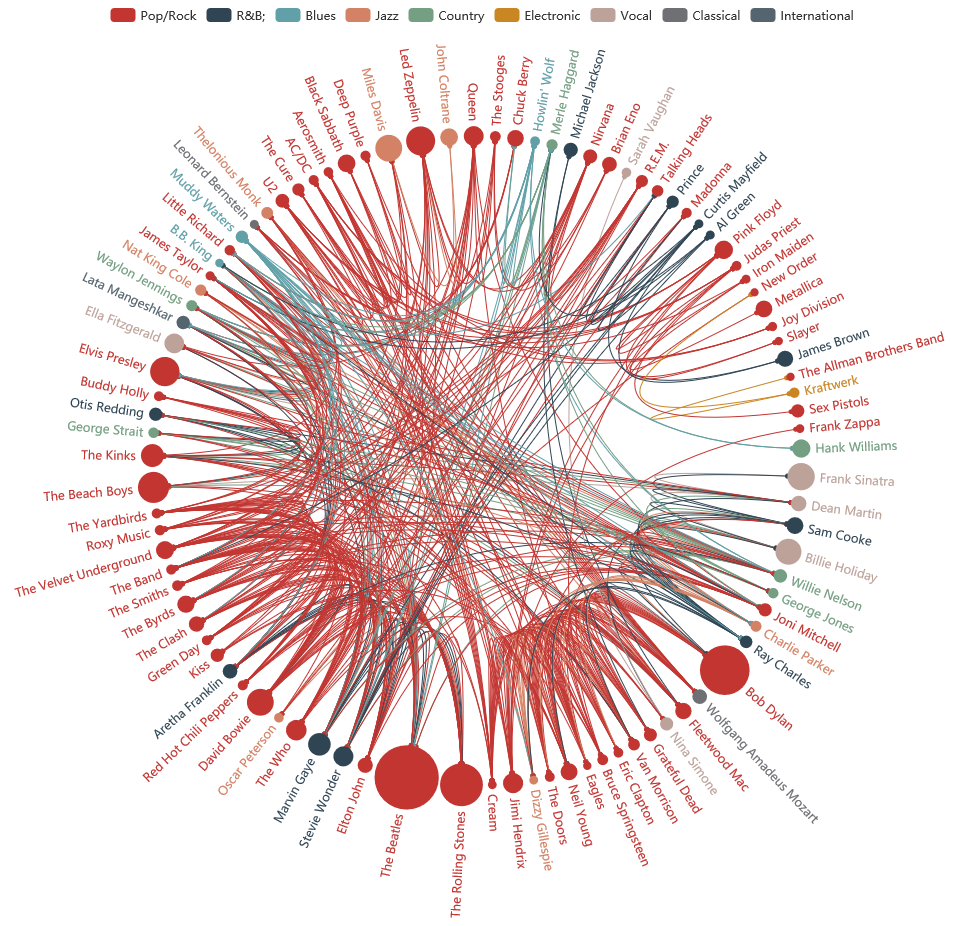
\includegraphics[width=1.25\textwidth]{figures/xdq/similarity.png}
\setlength{\leftskip}{0pt plus 1fil minus \marginparwidth}
\setlength{\rightskip}{\leftskip}
\caption{An influence network based on musical similarity}
\label{fig:similarity}
\end{figure}

\section{A comparison between two influence networks}

So far, two influence networks have been obtained. The first directed one (Figure \ref{fig:influence}) is reported by the artists themselves, as well as the opinions of industry experts. The latter one without arrows is established by the degree of similarity between song characteristics, such as structure, rhythm, or lyrics. We are curious about the difference between them, and hopefully we expect to find some interesting information. 

Generally speaking, most artists are mainly influenced by artists within the same genre as reported in the first network, while more between-genre-influence relationships are witnessed in the second network. This phenomenon is contributed to the subjectivity involved in the interviews or comments. Artists tend to claim they follow the famous musicians in the genre they belong to. In addition, industry experts often start from a professional manner to make judgements, that is to say, the genre barrier cannot be overlooked in this scenario.

To be specific, each artist has a list of ``nominal'' (self-claimed) followers and a list of potential professional fans (based on musical similarity). These two lists may overlap to some extend, indicating that a ``double-checked'' strong bond among artists exists.

For simplicity and convenience, the influence data of the famous artist Bob Dylan is taken as an example for analysis. Two mini influence networks related to Bob Dylan are shown in Figure \ref{fig:bob1} and \ref{fig:bob2}.

\begin{figure}[htbp]
    \setlength{\leftskip}{0pt plus 1fil minus \marginparwidth}
    \setlength{\rightskip}{\leftskip}
    \begin{subfigure}{0.5\linewidth}
        \centering
        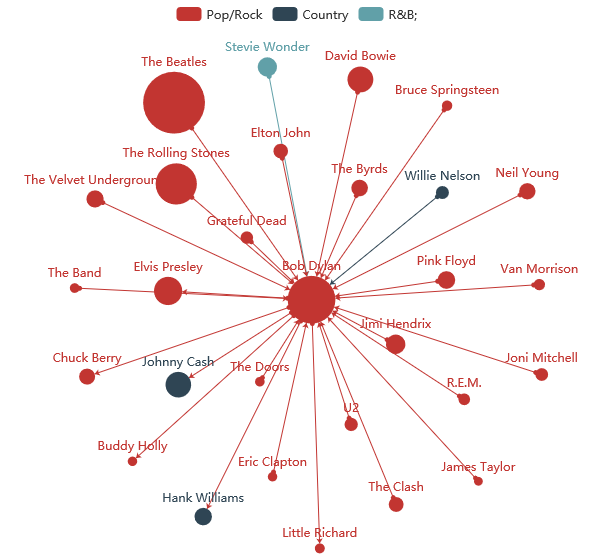
\includegraphics[width=\textwidth]{figures/xdq/BOB1.png}
        \caption{reported by artists \& experts}
        \label{fig:bob1}
    \end{subfigure}
    \begin{subfigure}{0.5\linewidth}
        \centering
        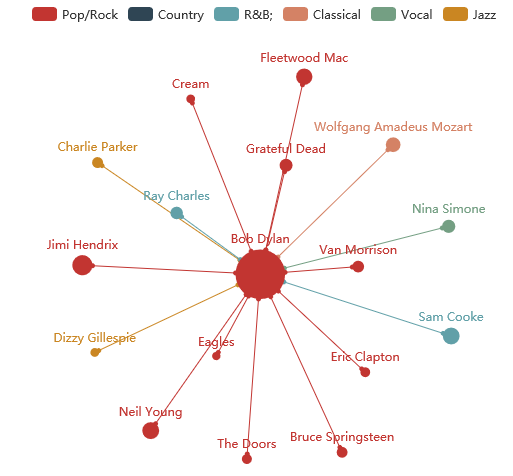
\includegraphics[width=\textwidth]{figures/xdq/BOB2.png}
        \caption{computed from similarity analysis}
        \label{fig:bob2}
    \end{subfigure}
    \caption{Bob Dylan influence networks}
\end{figure}


% \begin{figure}
% 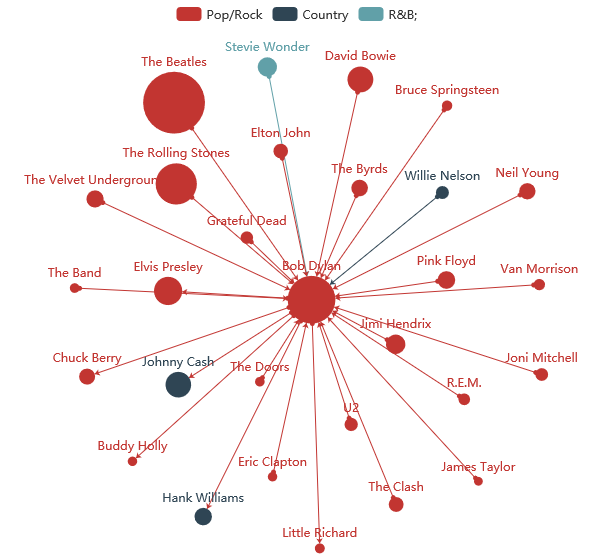
\includegraphics[width=0.5\textwidth]{figures/xdq/BOB1.png}
% \centering
% \caption{Bob Dylan influence network 1: reported by artists}
% \label{fig:bob1}
% \end{figure}

% \begin{figure}
% 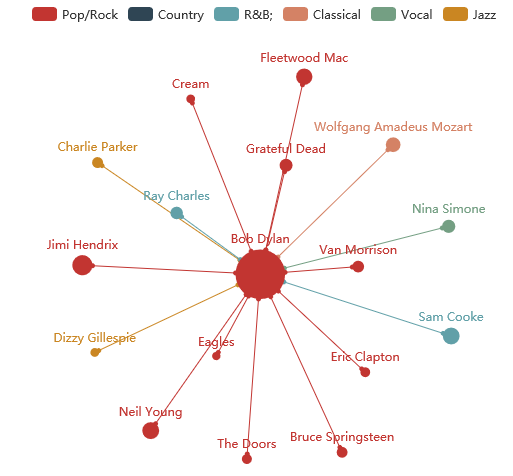
\includegraphics[width=0.5\textwidth]{figures/xdq/BOB2.png}
% \centering
% \caption{Bob Dylan influence network 2: from similarity analysis}
% \label{fig:bob2}
% \end{figure}

The left figure shows the artists that have influenced on or been influenced by Bob Dylan according to data reported by artists \& experts. The right one illustrates the artists sharing similar music features with Bob Dylan. 7 artists appear in both networks, indicating a strong influence --- not only orally judged by person, but also reflected in their musical works. They are: Grateful Dead,Van Morrison, Eric Clapton, Bruce Springsteen, Neil Young, The Doors and Jimi Hendrix. We also checked whether some self-claimed followers have a very different music style with their influencer, and the result shows that no one does.



% \begin{enumerate}
%     \item 谁才是Bob Dylan的忠实拥趸?
%     \begin{enumerate}
%         \item Grateful Dead
%         \item Van Morrison
%         \item Eric Clapton
%         \item Bruce Springsteen
%         \item Neil Young
%         \item The Doors
%         \item Jimi Hendrix
%     \end{enumerate}
%     \item 谁又与Bob Dylan的曲风大相径庭?
%      \begin{enumerate}
%         \item 《震惊,潮水退去,竟是他在裸泳!!!》
%         \item 《你为什么接受采访,你是不是有什么不可告人的目的?》
%         \item 《谁指使你这么说的?》
%         \item to be continued 2022.05.25
%     \end{enumerate}
% \end{enumerate}


% % test
% \begin{figure}
%     \centering
%     
% 定义流程图节点
\tikzstyle{startstop} = [
  rectangle,
  rounded corners,
  minimum width=2cm,
  minimum height=1cm,
  text centered,
  draw=black
]
\tikzstyle{io} = [
  trapezium,
  trapezium left angle=75,
  trapezium right angle=105,
  minimum width=1cm,
  minimum height=1cm,
  text centered,
  draw=black
]
\tikzstyle{process} = [
  rectangle,
  minimum width=2cm,
  minimum height=1cm,
  text centered,
  draw=black
]
\tikzstyle{decision} = [
  diamond,
  minimum width=2cm,
  minimum height=1cm,
  text centered,
  draw=black]
\tikzstyle{arrow} = [thick, ->, >=stealth]

\begin{tikzpicture}[node distance=2cm]
  % 设置节点
  \node (pic) [startstop] {待测图片};
  \node (bg) [io, below of=pic] {读取背景};
  \node (pair) [process, below of=bg] {匹配特征点对};
  \node (threshold) [decision, below of=pair, yshift=-0.5cm] {多于阈值};
  \node (clear) [decision, right of=threshold, xshift=3cm] {清晰?};
  \node (capture) [process, right of=pair, xshift=3cm, yshift=0.5cm] {重采};
  \node (matrix_p) [process, below of=threshold, yshift=-0.8cm] {透视变换矩阵};
  \node (matrix_a) [process, right of=matrix_p, xshift=3cm] {仿射变换矩阵};
  \node (reg) [process, below of=matrix_p] {图像修正};
  \node (return) [startstop, below of=reg] {配准结果};
    
  % 连接节点
  \draw [arrow](pic) -- (bg);
  \draw [arrow](bg) -- (pair);
  \draw [arrow](pair) -- (threshold);

  \draw [arrow](threshold) -- node[anchor=south] {否} (clear);

  \draw [arrow](clear) -- node[anchor=west] {否} (capture);
  \draw [arrow](capture) |- (pic);
  \draw [arrow](clear) -- node[anchor=west] {是} (matrix_a);
  \draw [arrow](matrix_a) |- (reg);

  \draw [arrow](threshold) -- node[anchor=east] {是} (matrix_p);
  \draw [arrow](matrix_p) -- (reg);
  \draw [arrow](reg) -- (return);
\end{tikzpicture}

%     \caption{Caption}
%     \label{fig:my_label}
% \end{figure}
